% !TeX root = ../thesis.tex
% TH-CH02-WRITE-V1: reviewed materials; draft, not compiled or frozen.
\chapter{机器人多任务仿真平台与触觉感知建模}
\label{chap:simulation_platform}

\section{系统需求与总体架构}
\label{sec:platform_architecture}

多任务灵巧手操作要求机器人在同一场景中完成接近、接触、抓持和物体运动等连续过程。机械臂决定手部能够到达的位置与姿态，欠驱动灵巧手通过有限驱动通道形成接触，触觉观测则反映接触发生后的局部响应。这些环节相互影响，因此需要在同一执行过程中联合描述运动、接触与观测。为支持后续专家示教生成与触觉数据研究，本文搭建RM75B机械臂与途见科技灵巧手仿真平台，将机器人模型、控制接口、触觉阵列、任务逻辑和记录模块组织到统一执行流程中。平台基于MuJoCo完成多刚体动力学和接触计算\cite{todorov2012mujoco}，本章说明各模块如何协同执行，以及触觉读数在该模型中的具体含义。

平台采用图\ref{fig:ch02_architecture}所示的五层结构。模型层保存机械臂、手部、底座及物体资产，负责提供关节和几何关系；控制层将动作解释为关节或末端目标；感知层在机器人表面配置触觉采样区域并组织观测；任务层设置场景、初始条件和评价逻辑；记录层保存执行过程中的状态、动作与传感器输出。各层通过明确接口组合，主要职责见表\ref{tab:ch02_modules}。这种组织方式使任务配置不必重复实现机器人模型，也使传感器后处理能够与任务成功条件分开检查。

\begin{figure}[htbp]
  \centering
  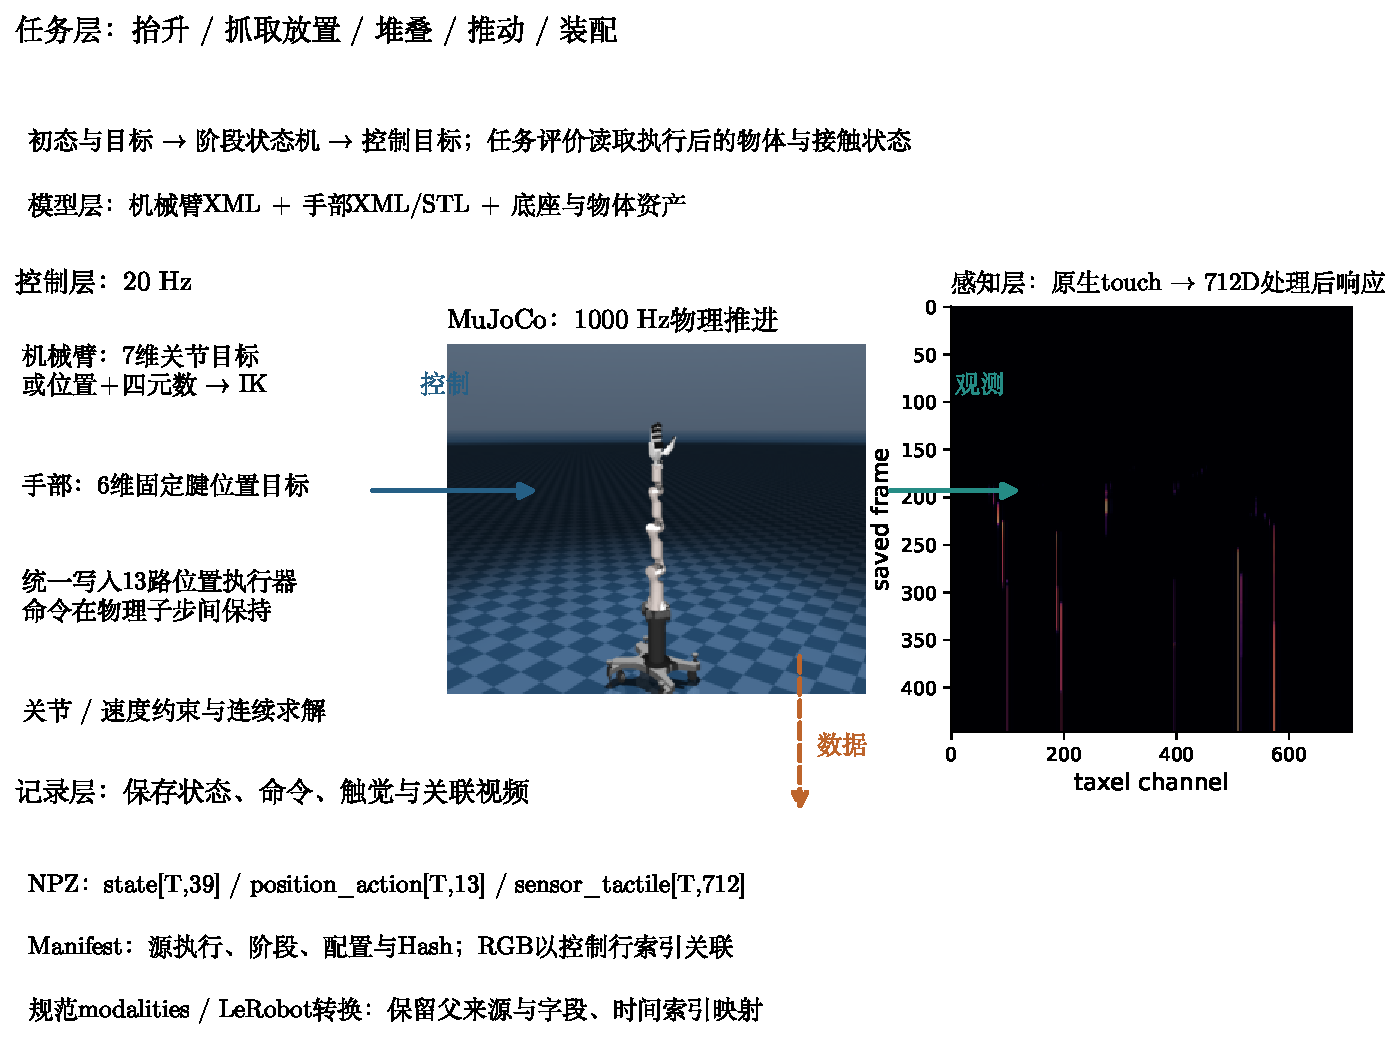
\includegraphics[width=0.97\textwidth]{figures/annotation_R2/platform_actual_architecture.pdf}
  \caption{仿真平台模块及控制、观测数据流}
  \label{fig:ch02_architecture}
\end{figure}

\begin{table}[htbp]
  \centering\small
  \caption{仿真平台主要模块与功能}
  \label{tab:ch02_modules}
  \begin{tabular}{p{0.15\textwidth}p{0.32\textwidth}p{0.39\textwidth}}
    \hline
    模块 & 主要组成 & 接口职责\\
    \hline
    模型层 & 模型描述、资产与组合构建器 & 确定关节、执行器、几何及安装关系\\
    控制层 & 机械臂与手部位置控制器 & 将动作转换为执行器控制量\\
    感知层 & 曲面阵列与信号处理器 & 绑定传感器地址并输出有序观测\\
    任务层 & 场景、任务状态与评价器 & 设置任务条件并评价执行状态\\
    记录层 & 在线记录及合同检查 & 保存关联记录并检查数组合法性\\
    \hline
  \end{tabular}
\end{table}

一次控制周期中，环境先将动作送入控制器，再推进若干物理子步，随后读取观测并进行任务评价。记录模块位于执行链路的接口处，不参与接触力求解。这样的顺序有助于区分控制目标、物理状态和观测结果，避免把目标动作直接当成已经完成的运动。

平台设置Lift、PickPlace、Stack、Push和NutAssembly五类任务接口，分别面向抬升、搬移放置、堆叠、推动和装配过程。任务工厂负责选择任务对象，并由任务实例补充相应场景。接口注册说明软件具有对应入口，但不能代替具体条件下的执行验证。本章仅以已有代表性记录核查观测输出，抓取生成与任务性能分析在第三章展开，数据组织及质量控制在第四章讨论。

\section{RM75B机械臂与途见科技自研灵巧手模型}
\label{sec:robot_model}

机器人组合模型选用与实验室设备型号对应的RM75B机械臂及途见科技自研欠驱动灵巧手，并通过底座和末端安装变换完成组合。XML规定关节、驱动和刚体连接，STL保存连杆与皮肤形状，URDF保留机构描述参考；当前构建器实际加载XML及其网格资产，统一模型接口。本文在该资产配置上研究控制与感知布局，几何尺寸误差、动力学参数和触觉响应的实机标定作为后续验证内容。机械臂采用MuJoCo模型描述格式（MuJoCo Modeling Format，MJCF），以XML文件组织刚体、关节、执行器和传感器。该模型定义七个串联转动关节，依次命名为joint1至joint7，其位置目标分别由pos\_joint1至pos\_joint7执行器接收。各关节的轴、范围与连杆变换由XML给定，控制器据执行器关联关系定位实际关节地址，而不是假定它们在状态数组中始终连续排列。七自由度结构为末端位姿调节提供冗余，但冗余自由度能否用于避碰或姿态优化，还取决于实际控制目标和求解约束，不能仅由关节数量推断。

机械臂各级连杆通过局部位置和四元数描述相对变换，末端定义right\_hand安装体和right\_hand\_site。安装体用于附着手部模型，末端site用于位姿读取及逆运动学计算，两者职责不同。组合构建器将手部安装到指定body，并施加机械臂描述中给定的附加旋转，其XYZ欧拉角为$(-90^\circ,-90^\circ,0^\circ)$。该旋转通过四元数参与坐标组合，必须与父body原有变换共同使用。因此，附加安装角不能直接解释为灵巧手在世界坐标系中的姿态。对于定义在几何局部坐标系中的点，其所属刚体坐标由旋转和平移共同确定；同样的变换规则也用于后续触觉采样点安装。

\begin{figure}[htbp]
  \centering
  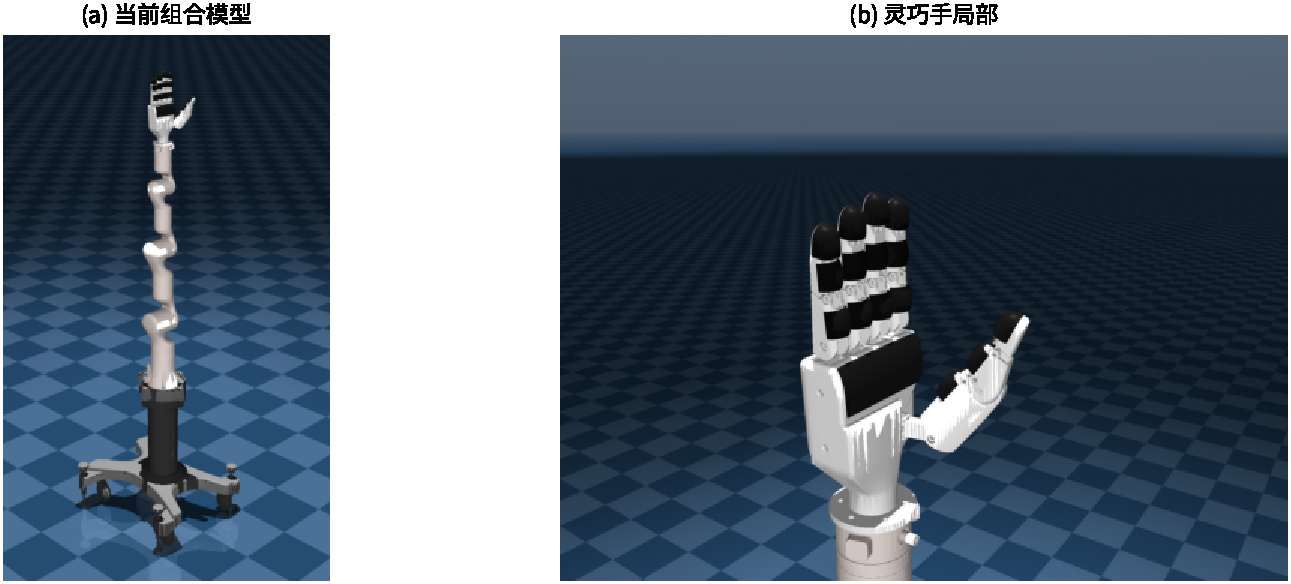
\includegraphics[width=0.96\textwidth]{figures/revision_20261127/robot_model.pdf}
  \caption{当前XML/STL模型的MuJoCo静态渲染：机械臂、底座与灵巧手组合及手部局部（关节零位）}
  \label{fig:ch02_robot_model}
\end{figure}

当前途见科技灵巧手模型含十二个转动关节，由六个固定腱和六个位置执行器驱动。其中四个手指分别具有两个转动关节，每指两个关节共同受一个屈曲腱驱动；拇指包含对掌关节及三个屈曲关节，对掌与屈曲分别对应一个驱动通道。手指上的三个触觉Patch不意味着三个独立关节：部分皮肤几何附着于同一指节刚体。模型需要分别记录机构自由度、执行器数量和感知区域数量，三者不存在一一对应关系。

固定腱通过关节坐标的线性组合定义传动长度，其关系写为
\begin{equation}
  l_t=\sum_{j\in\mathcal J_t}c_{tj}q_j,
  \label{eq:ch02_tendon}
\end{equation}
其中，$q_j$为第$j$个关节角，$\mathcal J_t$为第$t$个固定腱关联的关节集合，$c_{tj}$为XML中给定的传动系数。四指屈曲腱对两个关节均使用0.003的系数；拇指对掌系数为0.0085，屈曲腱的三个系数依次为0.0035、0.004和0.004。在模型长度约定下，控制目标对应腱坐标，不是各手指关节的独立角度目标。这些系数描述当前仿真传动，不作为实机推杆尺寸的测量结果。

\begin{figure}[htbp]
  \centering
  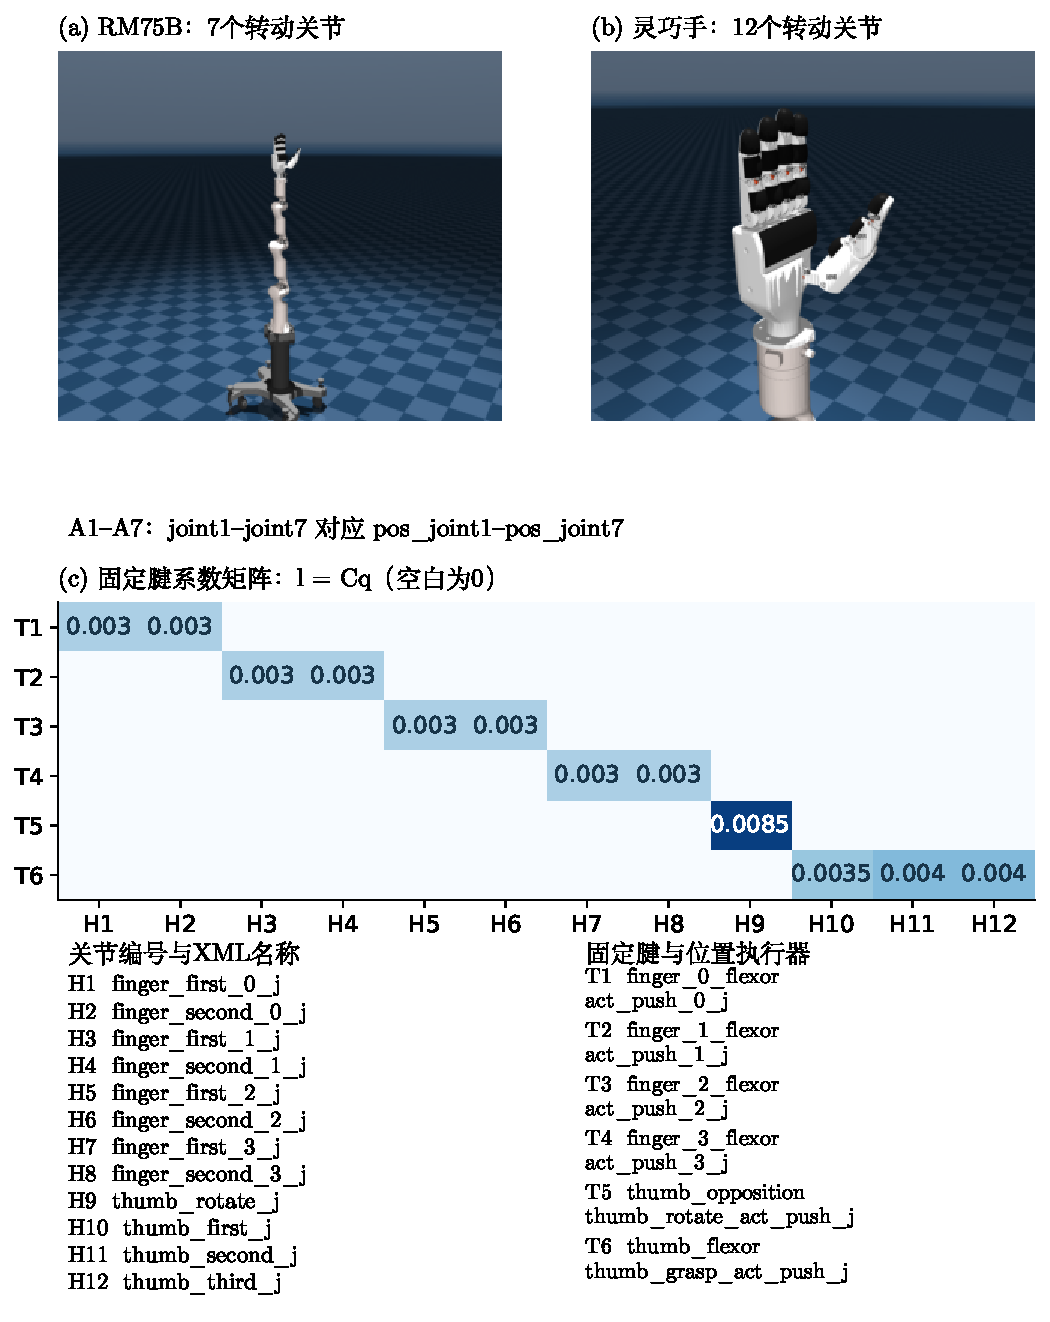
\includegraphics[width=0.97\textwidth]{figures/annotation_R2/joint_tendon_geometry.pdf}
  \caption{当前MuJoCo关节几何与XML固定腱系数、执行器对应关系}
  \label{fig:ch02_drive}
\end{figure}

\begin{table}[htbp]
  \centering\small
  \caption{机械臂及灵巧手执行器配置}
  \label{tab:ch02_actuators}
  \begin{tabular}{p{0.26\textwidth}p{0.23\textwidth}p{0.24\textwidth}p{0.13\textwidth}}
    \hline
    执行器或通道 & 控制坐标范围 & 比例增益$k_p$ & 输出限幅\\
    \hline
    pos\_joint1 & $[-3.1,3.1]$ rad & 5000 & $\pm60$ N$\cdot$m\\
    pos\_joint2 & $[-2.268,2.268]$ rad & 5000 & $\pm60$ N$\cdot$m\\
    pos\_joint3 & $[-3.1,3.1]$ rad & 3000 & $\pm30$ N$\cdot$m\\
    pos\_joint4 & $[-2.355,2.355]$ rad & 3000 & $\pm30$ N$\cdot$m\\
    pos\_joint5 & $[-3.1,3.1]$ rad & 2000 & $\pm10$ N$\cdot$m\\
    pos\_joint6 & $[-2.233,2.233]$ rad & 2000 & $\pm10$ N$\cdot$m\\
    pos\_joint7 & $[-6.28,6.28]$ rad & 1000 & $\pm10$ N$\cdot$m\\
    四指屈曲，各1通道 & $[0,0.01]$ m & 10000 & $\pm20$ N\\
    拇指对掌 & $[-0.0069,0.004]$ m & 4000 & $\pm20$ N\\
    拇指屈曲 & $[0,0.01]$ m & 4000 & $\pm20$ N\\
    \hline
  \end{tabular}
\end{table}

手部关节还配置被动弹簧及阻尼。驱动腱提供整体屈曲作用，而不同关节在接触物体后受到不同约束，未受阻关节仍可改变姿态，由此表达模型中的欠驱动适应行为。该机制并不意味着接触后每个关节都获得唯一稳定解，其运动还受弹簧、摩擦及求解参数影响。表\ref{tab:ch02_actuators}采用模型的SI单位约定：机械臂$k_p$单位为N$\cdot$m/rad，腱执行器$k_p$单位为N/m；腱力与关节力矩不能直接比较。这些是仿真参数，不是实物标定值。

手部采用刚体关节与固定腱传动描述欠驱动耦合，执行器通过腱长坐标同时作用于关联关节。模型的机构、安装变换和皮肤几何分别保存在XML、URDF与STL资产中。图\ref{fig:ch02_robot_model}展示安装后的组合模型与手部局部，图\ref{fig:ch02_drive}给出执行器、固定腱和关节之间的传动关系。

\section{灵巧手接触建模与控制方法}
\label{sec:contact_control}

本文实现组合位置控制器，将机械臂目标解释与手部腱驱动控制连接到MuJoCo执行器。设计中将目标求解放在控制周期内，将位置伺服与接触求解交由物理引擎执行：关节模式直接接收位置目标，末端模式先求解逆运动学，两者最终均输出七维机械臂关节目标；手部另接收六维腱位置目标。由此，同一套执行器接口可以服务于关节轨迹和末端轨迹，手部控制也保留其欠驱动传动关系。MuJoCo负责约束下的状态推进\cite{todorov2012mujoco,mujoco2026computation}，组合构建器统一采用Newton求解器、100次迭代上限、椭圆摩擦锥与0.001~s物理步长。

手部皮肤以mesh几何参与碰撞。padgeom默认接触维数为4，包括法向约束、两个切向滑动摩擦方向和绕接触法向的扭转摩擦方向，用于描述指面接触对滑移与转动的阻碍\cite{mujoco2026xml}。滑动、扭转和滚动摩擦配置值分别为1.3、0.02和0.0002；滚动摩擦方向在六维接触中使用，实际启用维数由接触配对规则确定。接触参考参数$(0.01,1)$采用正值格式，分别表示0.01~s时间常数和阻尼比1，用于设置约束恢复的柔顺性与阻尼。部分手指与拇指、手掌与手指之间另有显式pair，物体与桌面也有各自参数。碰撞求解采用皮肤mesh，感知布局则从同一资产派生采样点，两者分别承担接触计算与读出区域布置。

机械臂position模式将七维动作解释为关节位置目标，经合法范围约束后写入执行器控制数组。IK模式则接受末端位置与四元数组成的七维目标，在临时状态上迭代求解关节配置。设机械臂关节向量为$\boldsymbol q\in\mathbb R^7$，位置误差为$\boldsymbol e_p\in\mathbb R^3$，四元数误差转换得到的旋转向量为$\boldsymbol e_r\in\mathbb R^3$。代码分别调用末端site的位置与旋转Jacobian，按权重组成$\boldsymbol J_w$及$\boldsymbol e_w$。这里的旋转误差不是欧拉角逐分量相减，位置与旋转权重则用于调整两类误差在数值求解中的相对作用。

对加权Jacobian作奇异值分解后，控制器使用阻尼伪逆计算主任务修正，并在启用时叠加姿态项：
\begin{equation}
 \begin{aligned}
  \boldsymbol J_w&=\boldsymbol U\boldsymbol\Sigma\boldsymbol V^{\mathsf T},\qquad
  \boldsymbol J_{\lambda}^{+}=\boldsymbol V\,
  \operatorname{diag}\!\left(\frac{\sigma_i}{\sigma_i^2+\lambda^2}\right)
  \boldsymbol U^{\mathsf T},\\
  \Delta\boldsymbol q&=\boldsymbol J_{\lambda}^{+}\boldsymbol e_w+
  \left(\boldsymbol I-\boldsymbol J_{\lambda}^{+}\boldsymbol J_w\right)
  k_n(\boldsymbol q_0-\boldsymbol q).
 \end{aligned}
 \label{eq:ch02_ik}
\end{equation}
其中，$\sigma_i$为奇异值，$\lambda$为阻尼系数，$k_n$为姿态调节增益。默认开启零空间项且$k_n=0.1$；未显式指定时，$\boldsymbol q_0$取各关节执行器控制上下限的中点，当前机械臂对应七维零向量。阻尼能够限制小奇异值对应的更新放大，代码还依据奇异值和条件数调整阻尼。式\ref{eq:ch02_ik}中的第二项仅在零空间选项开启时使用；由于采用阻尼伪逆，其投影不应解释为对主任务完全无影响的严格正交零空间。另一个参数posture\_weight控制在误差与Jacobian中追加加权姿态残差，其默认值0仅关闭该附加残差，不关闭上述零空间项。式\ref{eq:ch02_ik}对应默认设置下SVD成功的路径；SVD失败时退回阻尼最小二乘求解，该分支不叠加零空间项。迭代达到位姿容差后可提前退出，所得目标还需进行关节限幅及速度平滑。指定profile采用position模式，不调用该IK求解路径。

\begin{figure}[htbp]
  \centering
  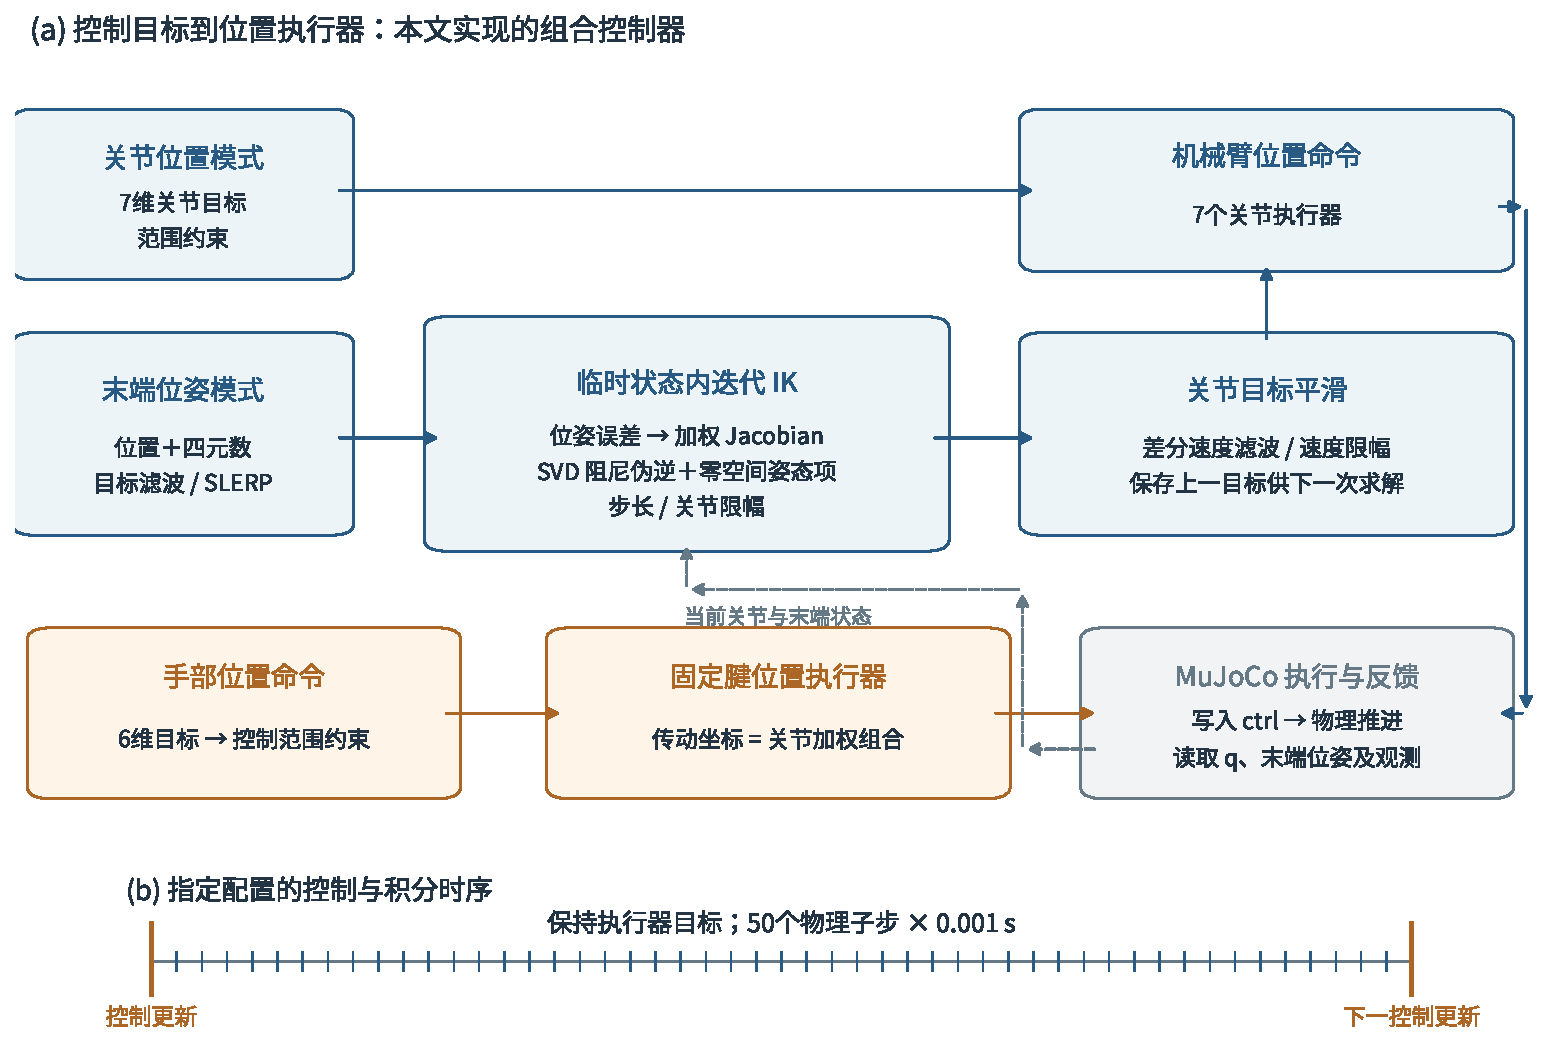
\includegraphics[width=0.97\textwidth]{figures/annotation_batch2/control_implementation.pdf}
  \caption{组合控制器的目标求解、执行器接口及多速率执行}
  \label{fig:ch02_control}
\end{figure}

\begin{table}[htbp]
  \centering\small
  \caption{主要控制与物理参数及其适用范围}
  \label{tab:ch02_control_parameters}
  \begin{tabular}{p{0.28\textwidth}p{0.23\textwidth}p{0.35\textwidth}}
    \hline
    参数 & 取值 & 配置层级\\
    \hline
    物理步长、求解器 & 0.001~s，Newton & 组合构建器覆盖值\\
    求解迭代上限、摩擦锥 & 100，椭圆锥 & 组合构建器覆盖值\\
    控制周期 & 0.05~s & 指定机器人profile\\
    IK迭代上限、初始阻尼 & 80，$10^{-3}$ & 控制器构造默认值\\
    位置、旋转误差权重 & 1，0.35 & 控制器构造默认值\\
    位置、旋转误差容差 & $10^{-4}$~m，$10^{-3}$~rad & 控制器构造默认值\\
    单次关节修正上限 & 0.15~rad & 控制器构造默认值\\
    目标关节速度上限 & 2~rad/s & 控制器构造默认值\\
    零空间调节增益 & 0.1 & 默认开启，可由调用方配置\\
    附加姿态残差权重 & 0 & 不影响零空间项的默认开关\\
    \hline
  \end{tabular}
\end{table}

图\ref{fig:ch02_control}给出两种机械臂模式及手部控制的汇合关系。IK求解在临时状态中迭代，以上一关节目标作连续求解初值，并在输出前进行速度滤波和限幅；实际仿真状态在随后的物理推进中更新。手部控制器接收六个位置通道，并根据执行器的传动类型读取坐标。固定腱执行器的位置由其关联关节的加权组合确定，控制器据此读取腱传动坐标，并与目标腱长比较。底层由MJCF位置执行器及其阻尼设置完成伺服，而不是在控制代码中另设一个通用力矩PD控制器\cite{mujoco2026xml}。表\ref{tab:ch02_control_parameters}列出控制器的默认参数，具体任务可在构造时覆盖。

指定profile的控制周期为0.05~s，环境按其与物理步长之比确定每周期50个子步，对应20~Hz控制和1000~Hz物理积分。图\ref{fig:ch02_control}中，动作只在控制周期开始时更新，执行器目标在子步内保持，环境完成物理推进后读取观测。物理积分频率决定状态推进间隔，观测采样频率决定保存时刻。接触可能在子步内出现或消失，因此20~Hz观测并不包含所有物理子步上的瞬态变化，这也是解释触觉时序时需要保留的采样边界。

\section{复杂曲面触觉阵列建模}
\label{sec:curved_tactile_array}

灵巧手指节和指尖具有不同曲率，直接在固定平面上均匀放置感知区域容易造成区域偏离表面、朝向不一致或局部重复覆盖。平台按实验室灵巧手的指节、指尖和手掌感知区域组织阵列，由相应皮肤STL派生采样点，再将局部位置与朝向安装到所属指节刚体。该建模过程使仿真感知区域随机构运动，并保留区域与通道的对应。阵列按手指与手掌的感知区域组织，使采样位置随各指节刚体运动，并保持固定的通道顺序。与以图像合成为主要输出的视觉触觉模拟器\cite{wang2022tacto,si2022taxim}不同，本平台在曲面附近布置原生touch感知区域，输出有序标量阵列。

每个手指设置近端、另一指节区域和指尖三个Patch，前两者为$4\times8$，指尖为$7\times8$；手掌设置$7\times16$阵列。五指共600个单元，手掌112个单元，总计16个Patch、712个感知单元。图\ref{fig:ch02_patch_order}按仿真索引展示布局组织，具体区间见表\ref{tab:ch02_patch_layout}。各区域的采样点分别由所属STL计算，以适应指节、指尖与手掌的曲率差异。

\begin{figure}[htbp]
\centering
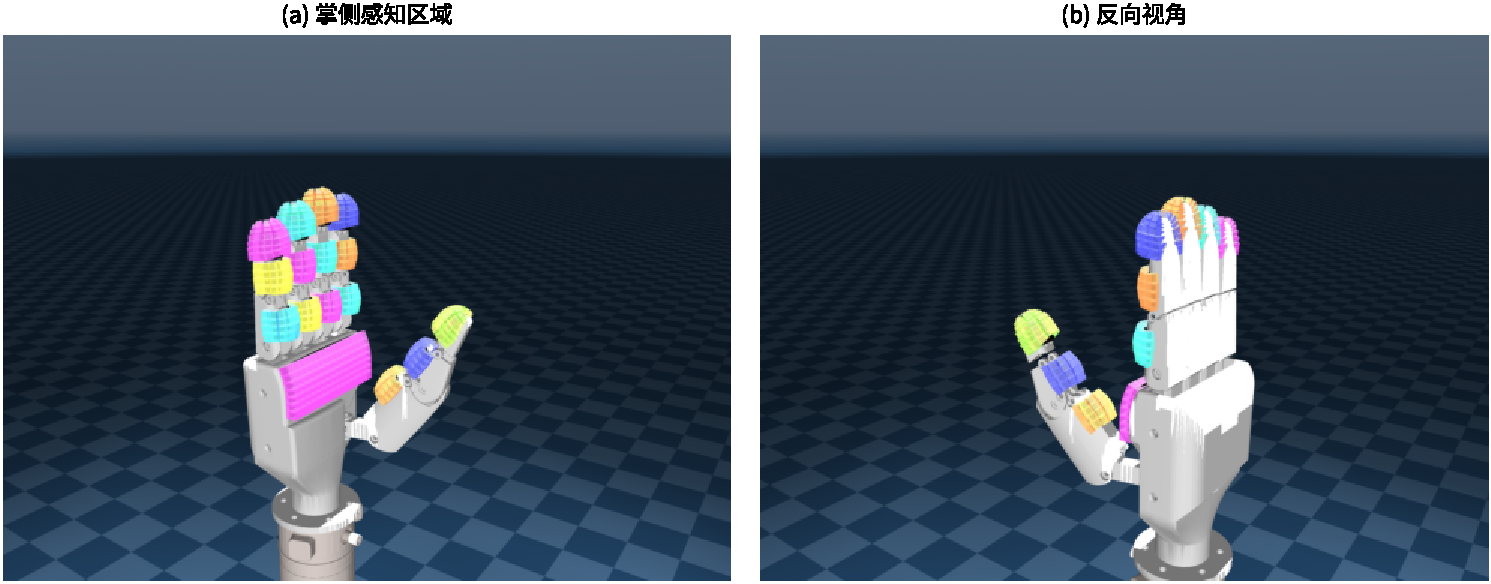
\includegraphics[width=0.97\textwidth]{figures/revision_20261127/tactile_layout.pdf}
\caption{当前MuJoCo模型中的16个Patch与712个box感知区域（颜色区分局部阵列）}
\label{fig:ch02_patch_order}
\end{figure}

segment策略面向指节皮肤。实现先对三角网格进行加密采样，通过主成分分析建立局部轴向与截面方向，再结合三角面朝向及径向分布筛选外表面。主成分方向来自几何点云的主要变化方向，并不自动具有固定的实物解剖含义。截面拟合和有效角度范围用于构造连续外壳样本，随后将样本组织成规则参数网格。与直接按原网格顶点布点相比，该过程能够减少三角网格局部密度差异对阵列索引分布的直接影响，但不保证最终点间距处处相等。

对规则外壳样本，程序拟合张量积Bezier曲面。设参数$u,v\in[0,1]$，控制点为$\boldsymbol C_{ij}\in\mathbb R^3$，曲面及其拟合关系为
\begin{equation}
 \begin{aligned}
  \boldsymbol S(u,v)&=\sum_{i=0}^{d_u}\sum_{j=0}^{d_v}
    B_i^{d_u}(u)B_j^{d_v}(v)\boldsymbol C_{ij},\\
  (\boldsymbol A^{\mathsf T}\boldsymbol W\boldsymbol A+\rho\boldsymbol I)\boldsymbol C
    &=\boldsymbol A^{\mathsf T}\boldsymbol W\boldsymbol P.
 \end{aligned}
 \label{eq:ch02_bezier}
\end{equation}
其中，$B_i^{d_u}$和$B_j^{d_v}$为Bernstein基函数，$\boldsymbol A$为采样参数对应的设计矩阵，$\boldsymbol P$存储三维样本，$\boldsymbol W$为样本权重。正则强度$\rho$由配置系数与加权设计矩阵的平均对角尺度共同确定，不能直接等同于配置中的无量纲系数。曲面坐标沿用网格的长度单位，参数坐标本身无量纲。最终Taxel位于参数单元中心，避免将相邻单元同时放到同一边界上。

指尖策略的配置名称为fingertip-ellipsoid，但当前函数体并非在理想椭球上直接布点。它先识别指尖的swept-shell外壳，分析轴向切片及外侧包络，再对规则样本拟合Bezier曲面。指尖拟合使用更高的轴向次数及边界权重，以表达末端弯曲和封闭区域；最终轴向参数在$[0.06,1]$范围分格后取中心，而不是把最后一行放到参数极点。这样能够避免指尖极点附近多列采样重合。



手掌采用mesh-uv策略。程序对网格进行PCA投影，在局部二维参数域内设置规则采样位置，再通过投影三角形的重心坐标插值恢复三维点。当多个表面投影重叠时，需要选择对应外表面；当采样位置落在投影缺口或边界之外时，使用实现中的最近三角形回退。该方法保留了采样点与网格的关系，但二维规则网格不等于曲面等面积划分，投影折叠和回退区域也可能产生不同的局部间距。表\ref{tab:ch02_layout_parameters}列出三类布局的关键差异，不能仅根据策略名称推断其几何性质。

图\ref{fig:ch02_fingertip}对照展示三类策略的代表形状：两个指节区域采用segment，指尖采用swept-shell外壳识别与Bezier拟合，手掌采用mesh-uv。各子图均使用对应STL和实际采样函数生成；灰色表示原始网格，橙色表示采样中心，连线仅表示阵列行列邻接。坐标沿用各网格局部坐标系，轴单位由米换算为毫米，各子图独立取尺度，不代表统一安装姿态或真实电极标定。
\begin{figure}[htbp]
  \centering
  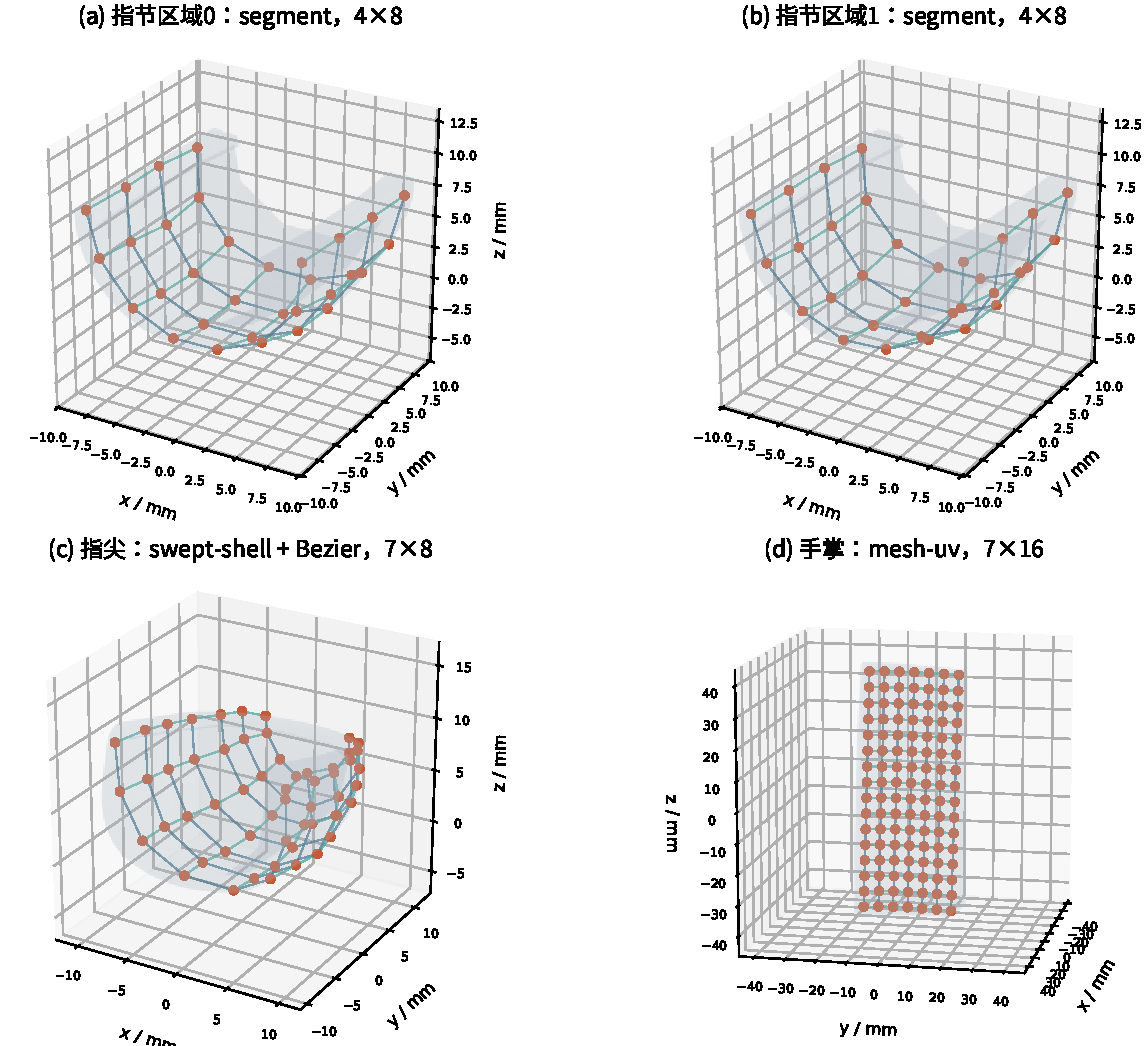
\includegraphics[width=0.97\textwidth]{figures/revision_20261127/surface_layout_strategies.pdf}
  \caption{三类曲面采样策略在指节、指尖和手掌代表网格上的布局（网格局部坐标）}
  \label{fig:ch02_fingertip}
\end{figure}


\begin{table}[htbp]
  \centering\small
  \caption{不同曲面布局方法的关键实现参数}
  \label{tab:ch02_layout_parameters}
  \begin{tabular}{p{0.18\textwidth}p{0.29\textwidth}p{0.39\textwidth}}
    \hline
    配置策略 & 外壳或参数域构造 & 拟合及最终采样\\
    \hline
    segment & PCA轴向、截面及外壳筛选 & Bezier次数$(5,7)$；正则系数$5\times10^{-5}$；参数单元中心\\
    指尖策略 & swept-shell外包络 & Bezier次数$(6,7)$；正则系数$8\times10^{-6}$；边界权重10\\
    mesh-uv & PCA二维投影 & 三角形重心插值；外侧选择与缺口回退\\
    \hline
  \end{tabular}
\end{table}

三类策略的区别来自表面几何：指节适合沿主要轴向组织截面，指尖需要处理封闭弯曲外壳与极点，手掌则通过投影三角形保留不规则网格。图\ref{fig:ch02_sampling_steps}给出实际采样函数的中间输出。指节和指尖先从STL识别密集外壳样本，再按各自Bezier配置拟合并取参数单元中心；手掌在PCA参数域设置格点，通过三角形定位与重心插值恢复三维位置。图中从原始几何到密集样本、再到最终阵列的变化，展示了规则索引如何依附不同曲面，而非将三种形状套用同一平面网格。

\begin{figure}[p]
 \centering
 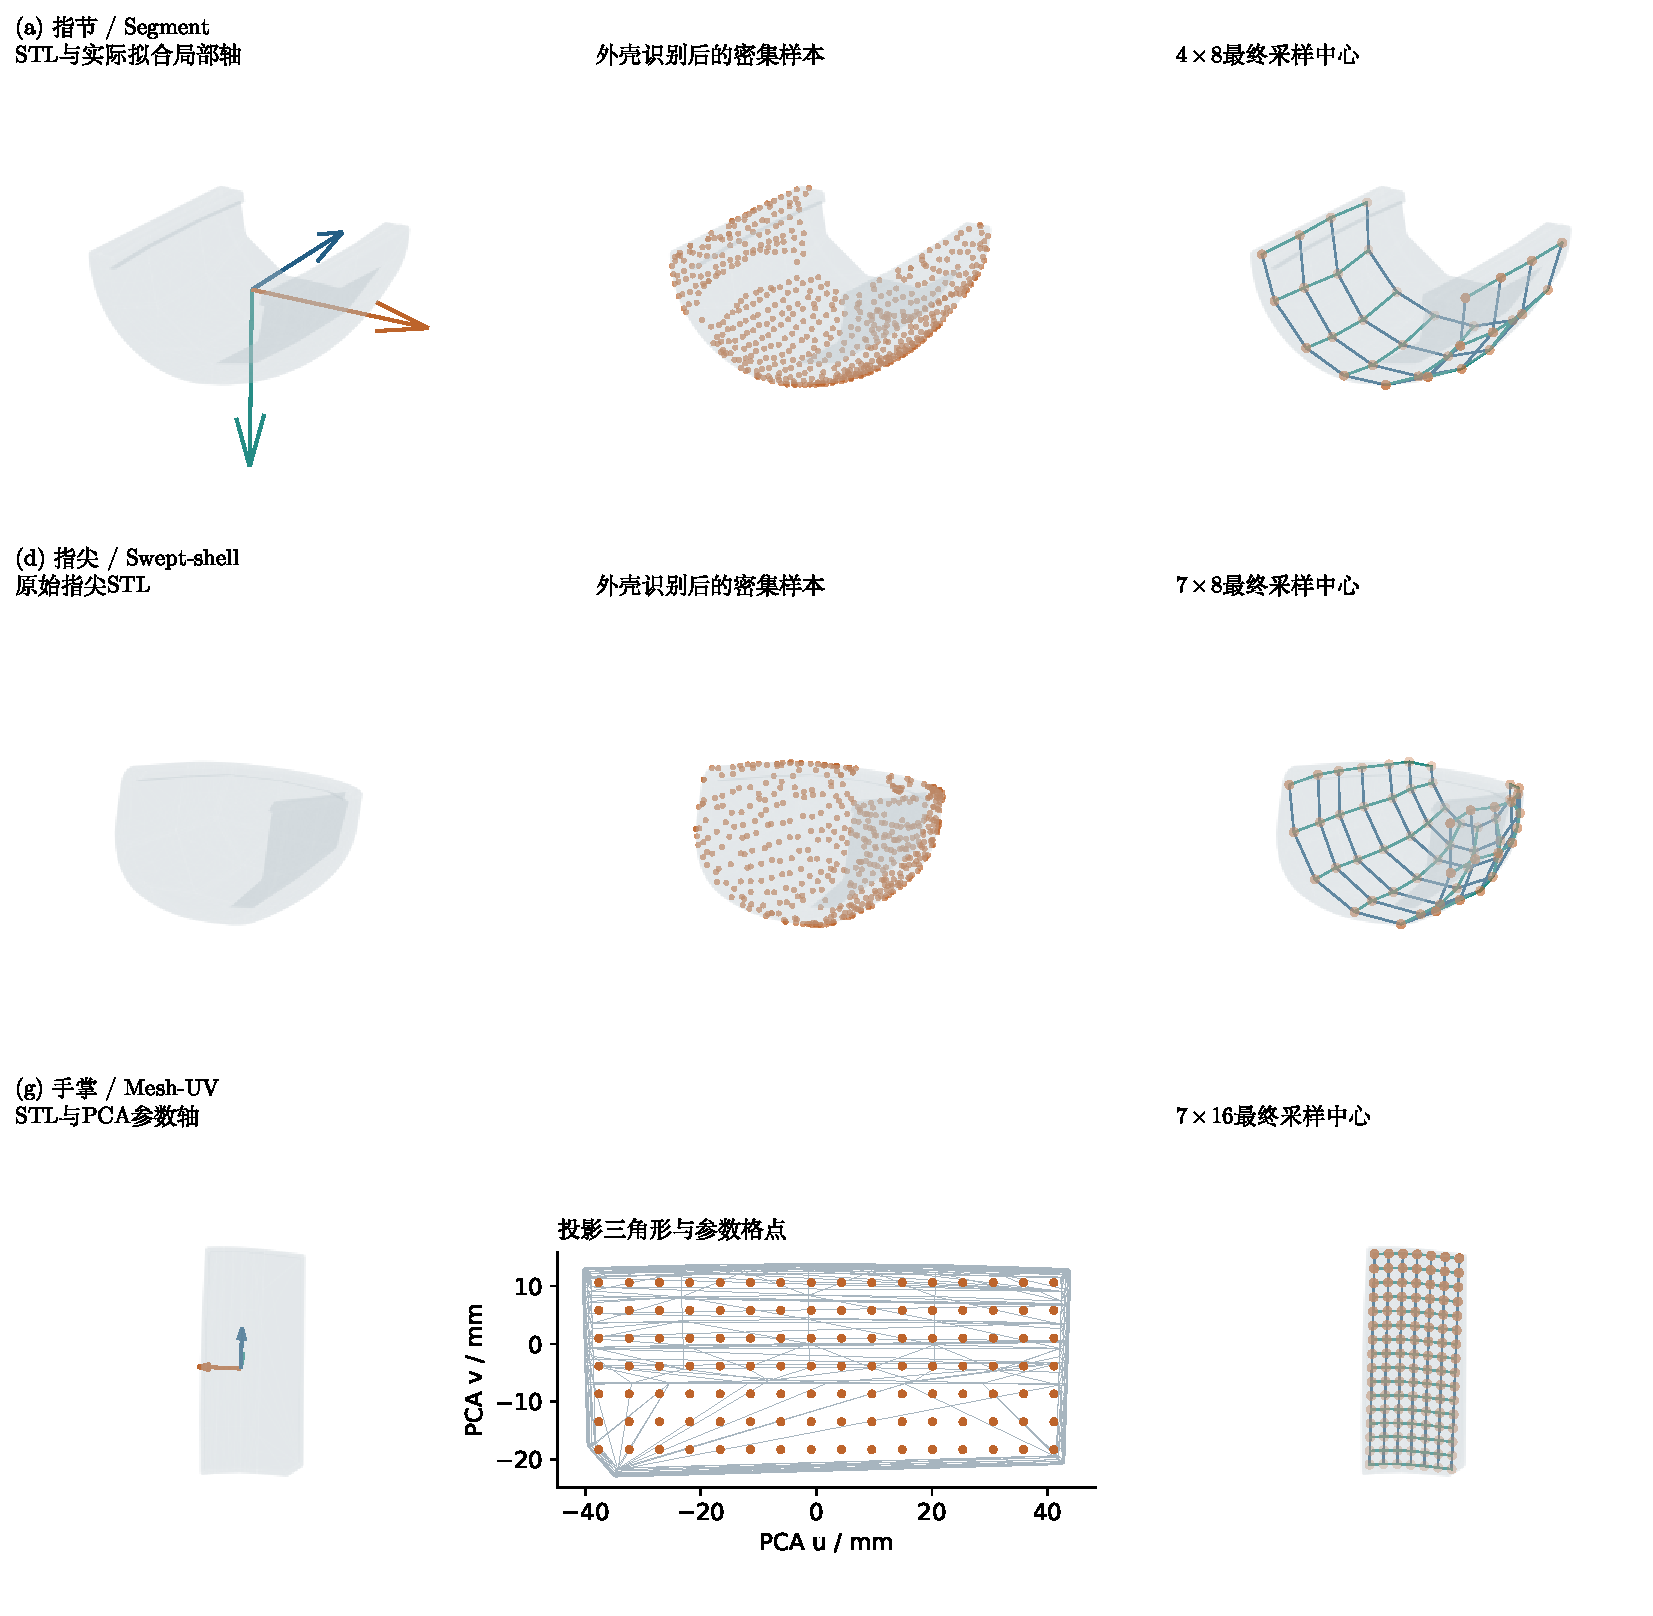
\includegraphics[width=0.98\textwidth,height=0.80\textheight,keepaspectratio]{figures/annotation_R2/sampling_processes.pdf}
 \caption{三类曲面采样的实际中间输出：STL与局部轴、外壳或参数域、最终采样中心}
 \label{fig:ch02_sampling_steps}
\end{figure}

对图中三个代表区域，最终采样点最近邻距离的最小值与中位数分别为：指节3.609/3.910~mm，指尖1.504/3.034~mm，手掌4.820/4.866~mm。距离按各点到其余采样点的最小欧氏距离计算，描述本次几何布局中的间距变化；曲率、感知区尺寸及接触覆盖还需结合各自模型分析。

网格采样点还需安装到正确的刚体上。程序先应用skin geom的局部旋转和平移，再根据行列相邻点差分构造切线。列方向归一化为$\boldsymbol e_x$，行方向经Gram--Schmidt正交化得到$\boldsymbol e_y$，法向由两者叉乘确定，局部方向矩阵为$[\boldsymbol e_x,\boldsymbol e_y,\boldsymbol n]$。随后依据点相对body或Patch参考位置进行外向修正。该步骤是保持感知区朝向一致的几何启发式，不能称为已经认证的实物表面法线。图\ref{fig:ch02_frame}展示局部切线与叉乘法向，特意区分外向修正前的坐标构造。

\begin{figure}[htbp]
  \centering
  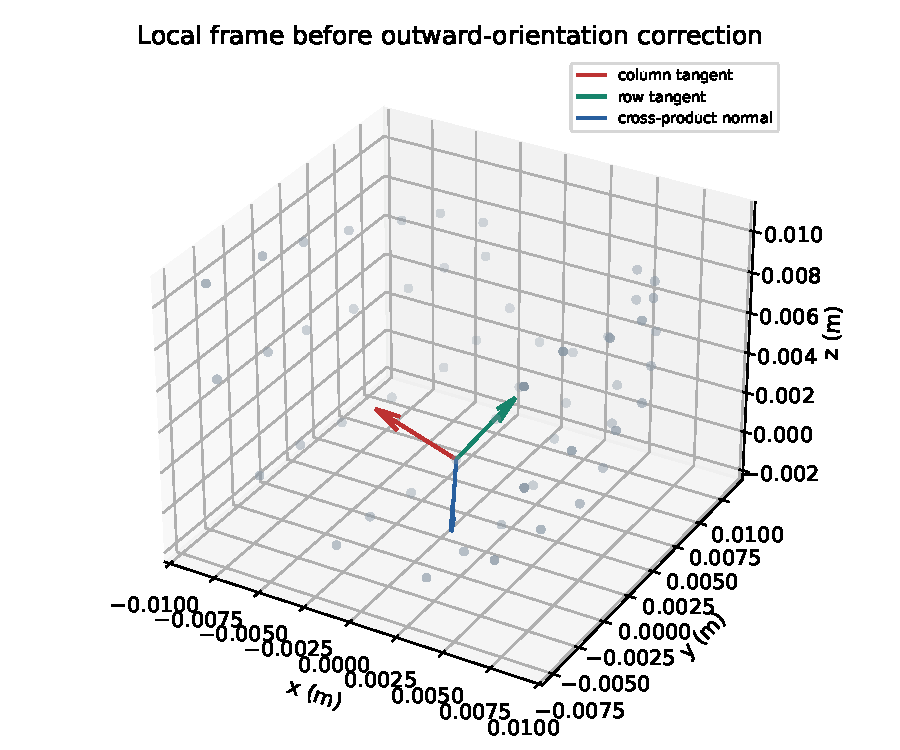
\includegraphics[width=0.66\textwidth]{figures/ch02/taxel_local_frame.pdf}
  \caption{由相邻采样点构造的局部切线和法向（外向修正前）}
  \label{fig:ch02_frame}
\end{figure}

每个采样点对应一个定向box site。其切向半宽分别依据列、行相邻距离设置：
\begin{equation}
 h_x=\max\!\left(h_{\min},\frac{\gamma d_c}{2}\right),\qquad
 h_y=\max\!\left(h_{\min},\frac{\gamma d_r}{2}\right).
 \label{eq:ch02_site_size}
\end{equation}
其中，$d_c,d_r$为对应方向可用相邻距离的最小值，$\gamma$为overlap系数，$h_{\min}$为最小半宽；法向半厚度$h_z$单独配置。指定profile取$\gamma=1.25$、$h_{\min}=0.0005$~m、$h_z=0.004$~m，而传感器类默认厚度和overlap分别为0.0015~m和1.0。二者必须按具体配置区分。box site用于指定有体积的感知区域，碰撞仍由皮肤几何参与计算；相邻感知区域允许重叠，以减少采样间隙。

\begin{table}[htbp]
  \centering\small
  \caption{16个Patch的阵列规格与712维索引区间}
  \label{tab:ch02_patch_layout}
  \begin{tabular}{llll}
    \hline
    Patch名称 & 行$\times$列 & 零基右开区间 & 布局类别\\
    \hline
    skin\_0\_0\_p & $4\times8$ & $[0,32)$ & segment\\
    skin\_0\_1\_p & $4\times8$ & $[32,64)$ & segment\\
    skin\_0\_2\_p & $7\times8$ & $[64,120)$ & 指尖策略\\
    skin\_1\_0\_p & $4\times8$ & $[120,152)$ & segment\\
    skin\_1\_1\_p & $4\times8$ & $[152,184)$ & segment\\
    skin\_1\_2\_p & $7\times8$ & $[184,240)$ & 指尖策略\\
    skin\_2\_0\_p & $4\times8$ & $[240,272)$ & segment\\
    skin\_2\_1\_p & $4\times8$ & $[272,304)$ & segment\\
    skin\_2\_2\_p & $7\times8$ & $[304,360)$ & 指尖策略\\
    skin\_3\_0\_p & $4\times8$ & $[360,392)$ & segment\\
    skin\_3\_1\_p & $4\times8$ & $[392,424)$ & segment\\
    skin\_3\_2\_p & $7\times8$ & $[424,480)$ & 指尖策略\\
    skin\_4\_0\_p & $4\times8$ & $[480,512)$ & segment\\
    skin\_4\_1\_p & $4\times8$ & $[512,544)$ & segment\\
    skin\_4\_2\_p & $7\times8$ & $[544,600)$ & 指尖策略\\
    skin\_palm\_p & $7\times16$ & $[600,712)$ & mesh-uv\\
    \hline
  \end{tabular}
\end{table}

阵列索引按手指0至4、每指Patch 0至2、最后手掌的顺序连接，各Patch内部采用行主序。索引顺序同时服务于传感器命名、观测展开与后处理还原，因而必须保持一致。该组织保证了仿真内部从曲面位置到数组通道的可追溯性，但不认证实机电气通道到同名索引的物理对应。后续展示触觉时可将区间恢复为原二维方阵，而不是把712个通道当作一条具有物理邻接关系的长序列。

曲面阵列的构建步骤归纳为算法\ref{alg:curved_tactile_build}。其输出为模型内的感知区域及传感器索引，不是独立碰撞单元或经标定的真实电极。
\begin{algorithm}[H]
\small
\caption{曲面触觉阵列构建}\label{alg:curved_tactile_build}
\KwIn{皮肤网格、所属刚体变换、16个Patch布局与尺寸配置}
\KwOut{712个box site、touch传感器及有序地址映射}
\ForEach{按既定顺序遍历的Patch $p$}{
读取对应STL及行列数，按配置布局策略计算曲面采样点\;
将网格坐标转换至所属刚体局部坐标，核对点数\;
\ForEach{按行主序遍历的采样点}{
由相邻差分构造切线并正交化，确定朝外局部坐标系\;
由邻域间距、overlap及最小半宽计算site尺寸\;
向所属刚体添加box site，并关联原生touch传感器\;
}
}
编译模型，绑定传感器地址并登记Patch索引区间\;
\end{algorithm}

\section{712维触觉观测及处理流程}
\label{sec:tactile_processing}

曲面布局确定感知区域的位置，触觉读出则决定每个区域记录什么量。构建器在组合手部之前调用传感器的augment\_spec接口，为每个采样点添加box site和一个MuJoCo原生mjSENS\_TOUCH传感器。模型完成构建后，bind依据传感器名称查找编号，检查输出维数为1，并保存sensor\_adr所指示的数据地址。地址与传感器编号不是同一概念，其他类型传感器可能占据不同长度的sensordata区间。read\_raw按已绑定地址读取712个值并转换为float32副本，避免后续物理更新改变已经返回的数组。

原生touch在相应body和site感知条件下累加接触法向力，输出非负标量\cite{mujoco2026xml}。在模型采用SI单位的约定下，它可解释为模拟法向力读数，但没有除以真实电极面积，也不包含完整切向力向量。一个接触可能被重叠感知区重复覆盖，因此全部Taxel读数求和不必等于机器人受到的总外力。该读出也不等同于视觉触觉图像或材料内部连续压力场\cite{si2022taxim,sferrazza2022simtoreal}。当前模型将上述box感知区域与原生touch逐一绑定，再按固定索引读取712维响应。

\begin{figure}[htbp]
  \centering
  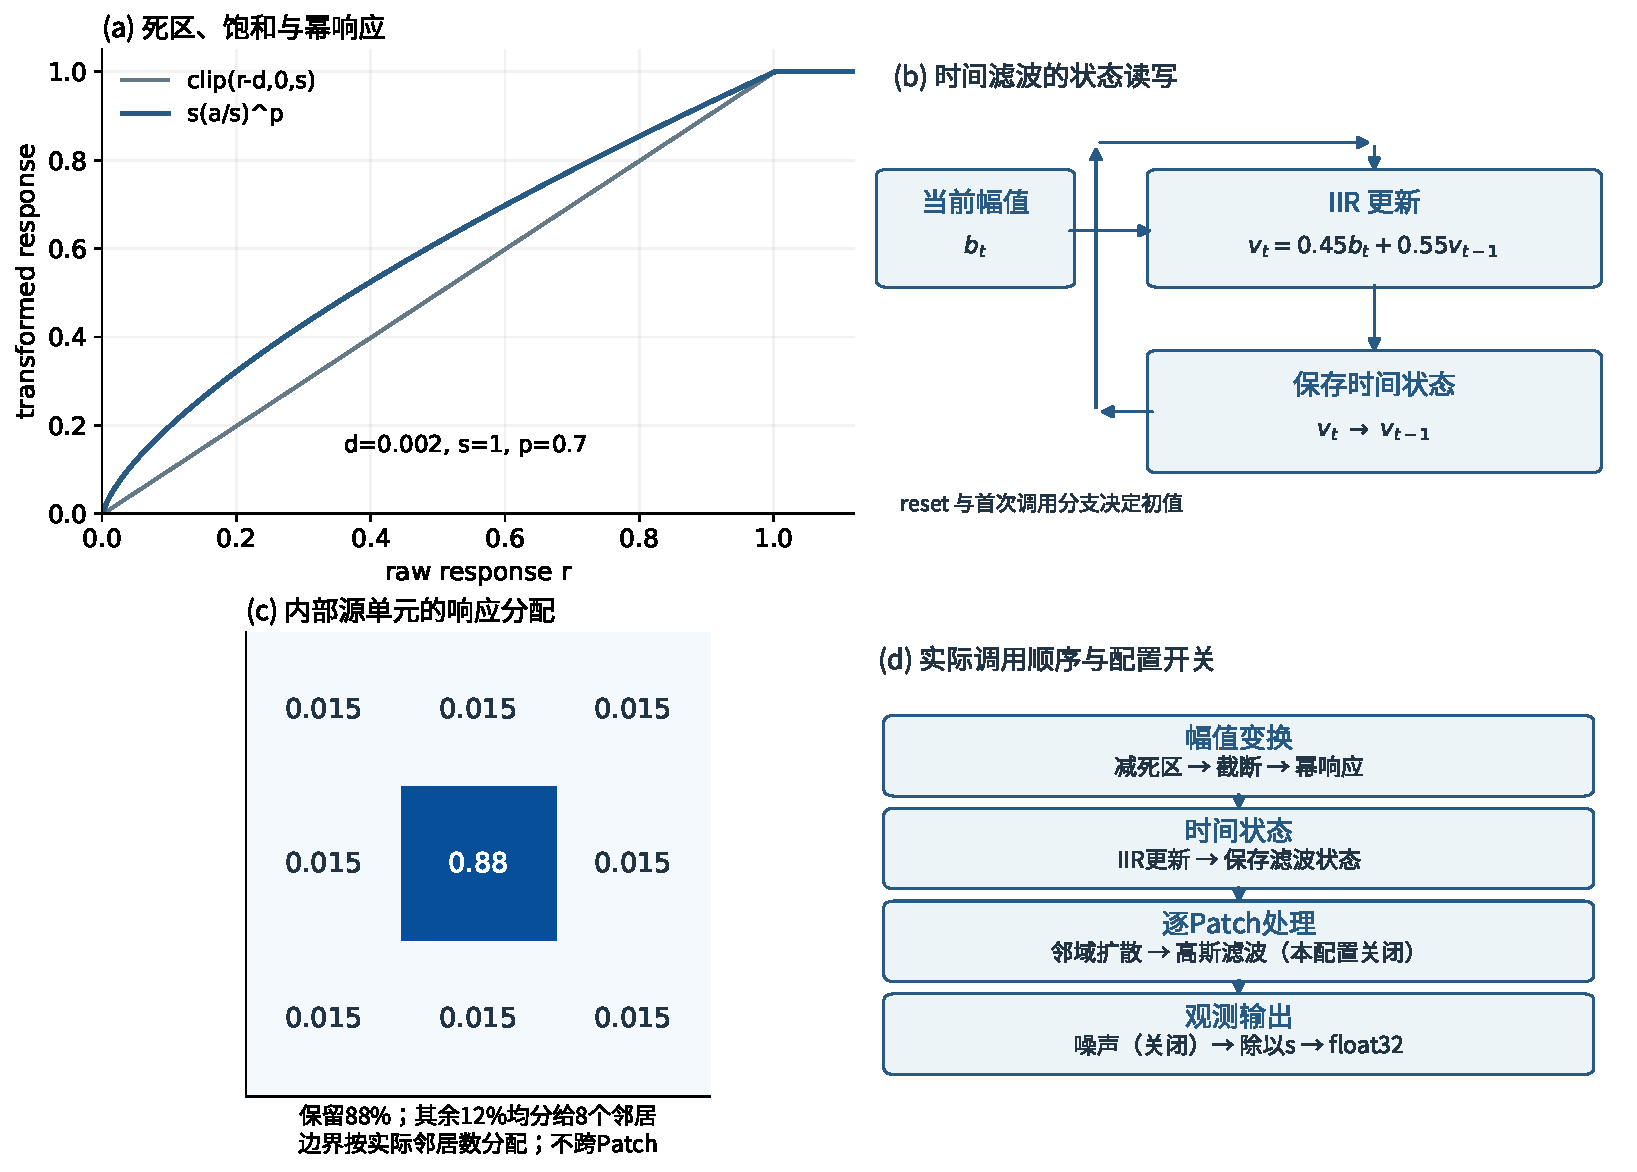
\includegraphics[width=0.97\textwidth]{figures/annotation_batch2/tactile_processing_operators.pdf}
  \caption{触觉幅值、时间与邻域处理算子及调用顺序（指定参数的公式示意）}
  \label{fig:ch02_processing}
\end{figure}

原始数组进入TactileSignalProcessor后，按图\ref{fig:ch02_processing}处理。设原始读数为$r_{t,j}$，死区为$d$，饱和尺度为$s$，幂指数为$p$，低通系数为$\alpha$，主要幅值处理写为
\begin{equation}
 \begin{aligned}
 a_{t,j}&=\operatorname{clip}(r_{t,j}-d,0,s),\qquad
 b_{t,j}=s(a_{t,j}/s)^p,\\
 v_{t,j}&=\alpha b_{t,j}+(1-\alpha)v_{t-1,j},\\
 \boldsymbol y_t&=\operatorname{float32}\!\left(
 \frac{\operatorname{clip}(\mathcal C_c(\boldsymbol v_t),0,s)}{s}\right).
 \end{aligned}
 \label{eq:ch02_processing}
\end{equation}
其中，$t$为连续调用的观测索引，$\mathcal C_c$为下述Patch内邻域扩散算子，$\boldsymbol y_t$为processed向量。末行适用于当前关闭高斯滤波和噪声、开启归一化的profile：先完成邻域扩散及范围限制，再除以饱和尺度$s$，最后转换为float32。滤波初态由处理器reset路径决定，不能假定任何数据片段都以相同方式独立初始化。指定profile使用$d=0.002$、$s=1$、$p=0.7$、$\alpha=0.45$，并开启归一化。死区和饱和设置改变了弱响应及尾部范围，幂变换与时间滤波又改变幅值和相邻观测关系，因此处理后的值不再保留原始模拟力的直接单位含义。

邻域扩散在每个Patch恢复的二维阵列中进行，用于将局部响应分配给邻近单元；图\ref{fig:ch02_processing}(c)显示内部源单元的分配权重。系数$c=0.12$表示每个源单元保留$1-c$的响应，其余部分按可用的8邻域数量平均分配。边界单元的邻居少于内部单元，程序按源单元归一化，不能写成所有接收单元统一除以8。邻域扩散只作用于同一Patch，数组中相邻但属于不同Patch的两个索引不会据此交换响应。当前profile的gaussian\_sigma和noise\_std均为0，高斯滤波与随机噪声属于可选能力，并未在该配置中启用。

\begin{table}[htbp]
  \centering\small
  \caption{触觉观测各阶段的输出与语义}
  \label{tab:ch02_signal_stages}
  \begin{tabular}{p{0.20\textwidth}p{0.27\textwidth}p{0.39\textwidth}}
    \hline
    阶段 & 维度或数据组织 & 处理及适用解释\\
    \hline
    空间布局 & 16个Patch、712个site & 定义感知位置、方向和体积\\
    原生touch & 每site一个非负标量 & 累加满足感知条件的接触法向力\\
    原始读取 & 712维float32副本 & 按sensor\_adr读取，顺序固定\\
    信号处理 & Patch方阵及时间状态 & 死区、截断、幂响应、IIR及邻域扩散\\
    processed输出 & 712维float32 & 指定profile归一化，无量纲响应\\
    \hline
  \end{tabular}
\end{table}

表\ref{tab:ch02_signal_stages}区分了几何采样、原生传感器值和后处理观测。最终向量保持表\ref{tab:ch02_patch_layout}的通道顺序，可还原为局部热图；热图色标只是显示方式，不改变原数组的物理语义。真实采集侧的processed还具有自身驱动和处理条件，不能仅凭同为712维就认为它与仿真观测单位相同。本文在后续跨域研究中保持这一区分，不将无量纲processed数据称为Pa或经过认证的真实压力。

\section{仿真平台功能验证}
\label{sec:platform_validation}

平台验证围绕模型接口、触觉读出和任务记录展开。模型与控制实现提供七个机械臂位置通道、六个手部腱驱动通道以及按传感器名称绑定的触觉地址；组合环境依次完成动作写入、物理推进、观测读取和任务评价。本节进一步分析五条保存的任务记录，检查触觉数组的形状、数值范围、采样时间与激活分布，并用原始视频说明相应操作场景。这样既能检验记录是否符合观测定义，也能观察接触响应在不同操作过程中的变化。

历史观测检查选择五任务开发记录中的五条代表性Episode，分别对应Lift、PickPlace、Stack、Push和NutAssembly。所读取对象为各案例source\_episode目录中的NPZ文件，并结合其manifest与结果记录确认任务来源。核查以完整保存数组为对象，不从中筛选有利时刻；统计字段固定为sensor\_tactile。设单条记录含$T$帧，则触觉合同要求数组为$T\times712$，数据类型为float32，所有元素有限且非负，同时检查是否全零。非零比例在整条数组上计算，用于描述保存响应的稀疏程度，不作为任务成功率或传感器准确率。

\begin{table}[htbp]
  \centering\small
  \caption{五条历史开发Episode的触觉观测核查结果}
  \label{tab:ch02_episode_validation}
  \begin{tabular}{lrrrr}
    \hline
    任务 & 帧数$T$ & 通道数 & 非零比例（\%） & 历史成功状态\\
    \hline
    Lift & 447 & 712 & 8.405 & True\\
    PickPlace & 638 & 712 & 15.296 & True\\
    Stack & 376 & 712 & 18.263 & True\\
    Push & 605 & 712 & 0.495 & True\\
    NutAssembly & 599 & 712 & 12.718 & True\\
    \hline
  \end{tabular}
\end{table}

图\ref{fig:ch02_historical_heatmaps}展示同一批记录的完整触觉序列。横向保留712个通道的原始顺序，纵向为记录帧索引，白线分隔16个感知区域。五条记录采用相同色标，能够同时观察响应出现在哪些通道、持续多少帧及其幅值变化。例如，推动记录的响应集中于少量通道，堆叠记录的激活范围更广；具体非零比例见表\ref{tab:ch02_episode_validation}。此处热图使用保存的处理后仿真响应，坐标为通道索引与帧索引。

\begin{figure}[htbp]
  \centering
  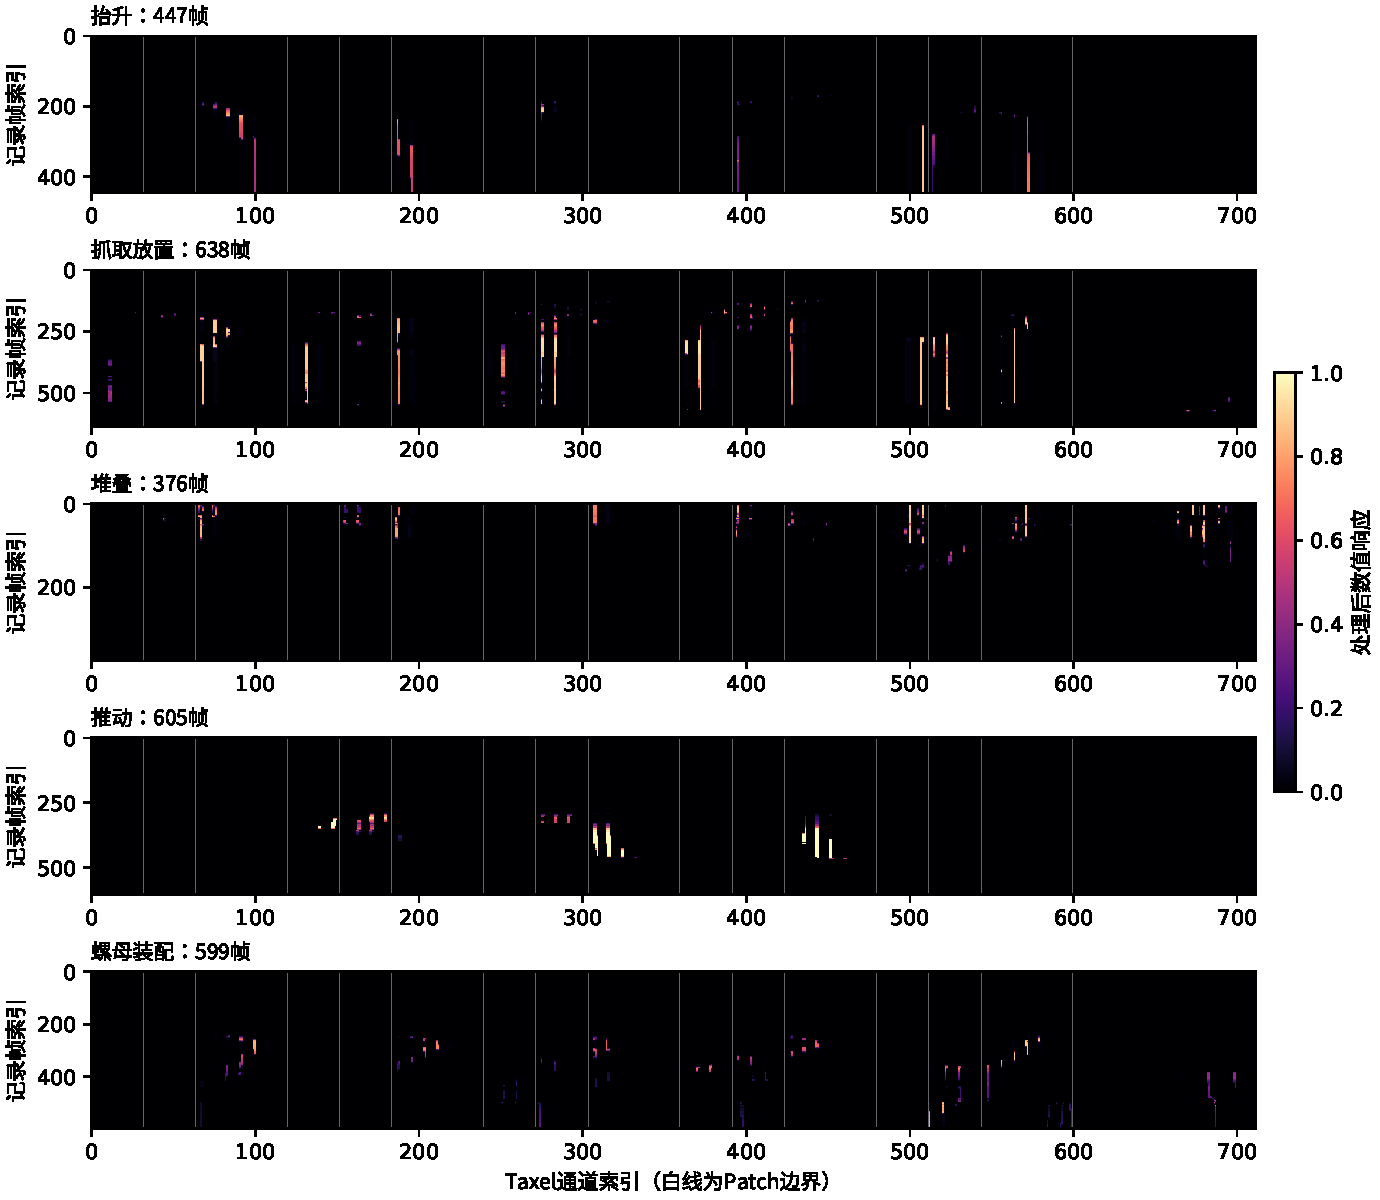
\includegraphics[width=0.96\textwidth]{figures/annotation_r2/historical_tactile_heatmaps.pdf}
  \caption{五条历史任务记录的处理后触觉热图（共用数值色标）}
  \label{fig:ch02_historical_heatmaps}
\end{figure}

表\ref{tab:ch02_episode_validation}中的五条触觉数组均为float32，满足$T\times712$的形状要求，所有元素有限、非负且存在非零响应。保存的float64时间戳相邻增量在浮点误差范围内为0.05~s，与20~Hz采样一致。触觉序列因此可以按记录索引分析接触响应的出现、持续和变化。

Push记录的非零比例为0.495\%，Stack为18.263\%。结合热图可以看到，推动记录仅在少量通道与时刻出现响应，堆叠记录的激活范围和持续阶段则更广。两者提示数据处理中应保留稀疏接触与较密集接触，而不以统一非零比例筛选所有任务。上述差异对应具体物体、轨迹及处理条件；每类一条记录用于展示观测特征，任务总体分布仍需按独立执行来源汇总。

五份NPZ同时保存tactile和sensor\_tactile，二者数值存在差异。本节按记录合同统一使用sensor\_tactile计算非零比例。两个字段的具体关系取决于相应版本的采样时刻与处理调用，现有检查尚未定位该差异的完整来源。

本节的证据范围为五条历史开发记录：其manifest及结果文件登记任务成功状态为True，Lift另有Strict严格轨迹回放记录。本文据保存数组分析触觉观测，未重新执行这些任务。历史记录与当前XML、曲面拟合和处理配置的完整版本对应关系为UNKNOWN；其独立来源还需结合初态分组（Root）与轨迹派生关系确定。相应统计分别保留帧数、执行记录及来源分组，以便后续数据审查。

上述检查确认了平台的模型、控制和观测接口，以及五条指定历史记录的数组有效性与基本采样关系。抓取候选如何转化为稳定操作，是下一章的研究问题；第四章则进一步检查这些执行记录的时序、来源及数据质量。真实触觉标定与跨域物理对应将在触觉重建的问题定义中统一讨论。

五类任务使用桌面、机器人及任务对象组成场景，初始条件由物体位姿、手部配置和目标区域确定。Lift以桌面物体为对象，依次接近、闭合、保持和抬升，任务接口按物体高度判断抬升结果；严格示教另检查尾段稳定性。PickPlace增加目标区域，抓持后运输、下降、释放并检查物体进入目标且手部离开。Stack在场景中增加支撑物，搬移目标物体到支撑面，释放后检查物体间接触与持续稳定。Push在桌面支撑下建立手物接触，反馈推动至目标区域，并检查位置、竖直范围与平面速度。NutAssembly场景包含待操作件与固定装配结构，抓持后调整姿态、运输和下降，按具体几何版本检查对准、插入及稳定状态。表中历史案例对应Sugar Box抬升、Tomato Soup Can搬移与推动、Stacking Ring堆叠及保留抓持命令的装配记录；各历史结果按自身manifest和版本解释，当前接口用于说明任务定义。

五类任务分别考察抓持后的垂直抬升、搬移与放置、物体堆叠、桌面推动以及螺母装配。图\ref{fig:ch02_historical_scenes}从上述五条记录的原始场景视频中提取首帧与末帧，展示物体、机械臂和灵巧手的相对位置及场景变化。起终帧用于说明各任务的操作对象与环境，任务结果仍按相应执行记录和验证条件判定。各任务的轨迹构建与执行条件在第三章进一步介绍。

\begin{figure}[p]
  \centering
  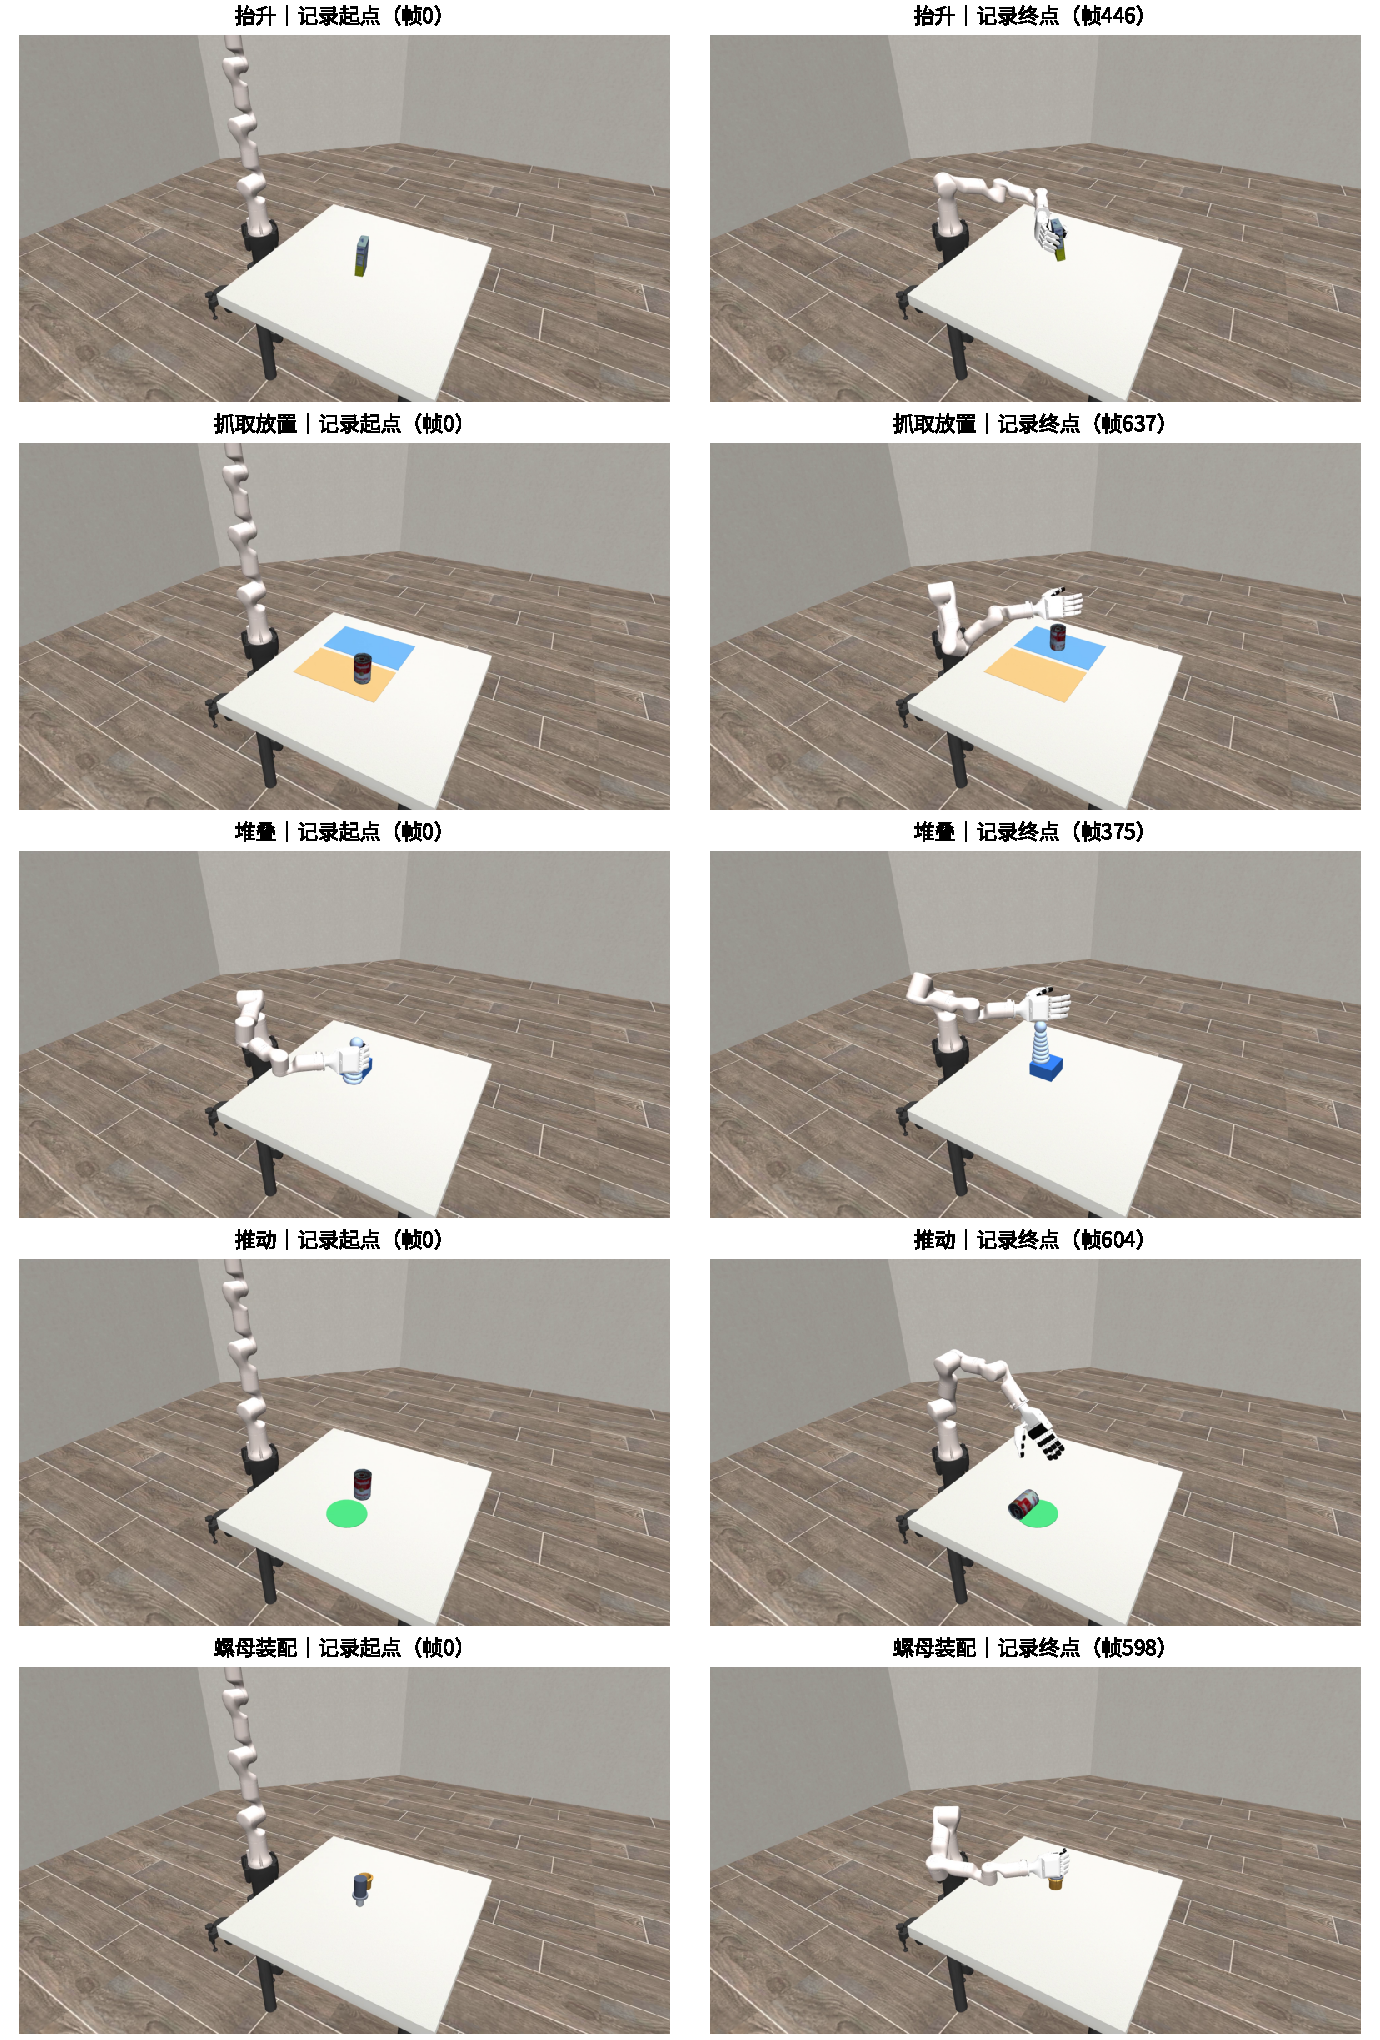
\includegraphics[width=0.92\textwidth,height=0.83\textheight,keepaspectratio]{figures/annotation_r2/historical_five_task_scenes.pdf}
  \caption{五任务历史仿真场景的记录起点与终点（原始视频帧）}
  \label{fig:ch02_historical_scenes}
\end{figure}

\section{本章小结}
\label{sec:platform_summary}

本章围绕多任务灵巧手操作的执行与感知需求，介绍了RM75B机械臂与途见科技灵巧手仿真平台的模型、控制、触觉、任务和记录接口。当前机械臂采用七个转动关节及位置执行器，手部采用十二个转动关节、六个固定腱和六个位置驱动通道。通过区分物理关节、传动坐标与控制通道，明确了欠驱动结构的实现范围，避免将历史命名中的推杆与当前机构混同。

控制过程区分关节目标或末端IK求解、底层位置伺服和物理积分，在指定配置下按20~Hz控制和1000~Hz积分执行。触觉阵列由皮肤STL派生，通过指节与指尖外壳拟合、手掌参数域投影及局部坐标构造形成16个Patch，再由712个原生touch感知区读取标量响应。死区、幂响应、时间滤波和邻域扩散进一步产生无量纲processed观测，其含义不同于经过标定的真实压力。

已有五条历史任务记录提供了触觉数组有限、非负和规则时间索引的功能证据，但与当前模型的完整版本一致性、独立Root关系及实物映射仍有限制。基于这些边界，下一章讨论如何将几何抓取候选转化为满足机械臂可达性、连续运动和任务要求的专家示教。
